\section{Zone Air Mass Flow Conservation}\label{zone-air-mass-flow-conservation}

\subsection{Overiew}\label{overiew}

The zone air mass flow conservation object, ZoneAirMassFlowConservation, activates zone air mass flow balance calculations. This feature is available only for controlled zones (ZoneVAC:EquipmentConnections) which also have either a zone mixing or infiltration object. The user may specify that zone mixing, infiltration, or both can be overridden to balance the zone air mass flows. The following rules apply:

\begin{itemize}
\tightlist
\item
  If there are no zone mixing flows to adjacent zones, then the zone air mass flow is balanced by setting the Zone Mixing objects mass flow rate to zero.
\item
  If there are no zone exhaust fans defined and there are no zone mixing objects specified, then a zone in an air loop is always balanced.
\item
  Infiltration mass flow is included in the zone air mass flow balance depending upon one of three options: none (all infiltration is assumed to be self-balanced), all zones, or only zones that serve as a source zone for zone mixing objects.
\item
  The base infiltration mass flow rate (calculated based on user inputs) may be controlled one of two ways for zone air mass flow balance purposes: adjust the base infiltration up or down as needed to balance the zone air mass flow, or assume the base infiltration rate is self-balanced and add infiltration if needed to balance the zone air mass flow.
\item
  Optional user inputs can override the default return air flow rate.
\end{itemize}

The zone air mass flow conservation equation always includes: supply air flow rates, return air flow rates, and zone exhaust fan flow rates. Zone mixing and infiltration object flow rates may be included depending upon the selected options. A particular zone can be a source zone, receiving zone, or both depending on the number of ZoneMixing objects specified for that zone.

\subsection{Return Air Flow Rate Calculations}\label{return-air-flow-rate-calculations}

The return air flow rate is calculated one of several ways, depending on whether ZoneAirMassFlowConservation is active, if there is more than one return node, and if Zone Return Air Node 1 Flow Rate Fraction Schedule Name or Zone Return Air Node 1 Flow Rate Basis Node or NodeList Name has been specified.


\subsubsection{Base Zone Total Return Flow}\label{base-zone-total-return-flow}

The total zone return flow calculation with no ZoneAirMassFlowConservation is the sum of the zone inlets less the sum of the zone exhausts adjusted for any balanced exhaust fan flow:

\begin{equation}
{\dot m_{R}} = MAX\left( {0.0,\,{{\dot m}_S} - [{{\dot m}_{EX,tot}} - {\dot m_{EXF,bal}}]} \right)
\end{equation}

If ZoneAirMassFlowConservation is active, then the total zone return air flow rate is 
\begin{equation}
{\dot m_{R}} = MAX\left( {0.0,\,{{\dot m}_S} - [{{\dot m}_{EX,tot}} - {\dot m_{EXF,bal}}] + [{{\dot m}_{XR}} - {{\dot m}_{XS}}]} \right)
\end{equation}

Note that the exhaust fan balanced flow component is not required to enforce the zone air flow balance when ZoneAirMassFlowConservation is active. 

\subsubsection{Zone Return Air Node 1}\label{zone-return-air-node1}

The first return air node is treated differently to maintain backward compatibility. If one or more Zone Return Air Node 1 Flow Rate Basis Nodes are specified in the ZoneHVAC:EquipmentConnections object, then the mass flow rate for the first return air node is:

\begin{equation}
{\dot m_{R,1}} = ReturnFlowSchedule*\sum\nolimits_j {{{\dot m}_{BasisNode,j}}}
\end{equation}

If there is only one return node and no Zone Return Air Node 1 Flow Rate Basis Nodes, then:

\begin{equation}
{\dot m_{R,1}} = ReturnFlowSchedule*{\dot m_{R}}
\end{equation}

In the zone air mass flow conservation calculation, the calculated zone total return flow rate is modified using return node flow schedule value when the zone air flow balancing is enforced and assigned to return node 1.  

\begin{equation}
{\dot m_{R,1}} = ReturnFlowSchedule*{\dot m_{R}}
\end{equation}

The zone air mass flow conservation calculation also limits the zone return node air flow rate with air loop design supply to protect from large number the solution may throw as follows:

\begin{equation}
{\dot m_{R,1}} = MIN\left( {{\dot m_{R,1}},\,{{\dot m}_{DesSupply,i}}} \right) 
\end{equation} 

\subsubsection{Allocation to Multiple Return Nodes}\label{allocation-to-multiple-return-nodes}

If there are multiple return air nodes in the zone, then each return air node is assumed to be paired with one supply air inlet node. The initial flow rate at a given return air node is based on the supply air inlet node for the same airloop and the AirloopHVAC Design Return Air Flow Fraction of Supply Air Flow:

\begin{equation}
{\dot m_{R,i}} = {DesignReturnFrac_i} * {\dot m_{S,i}}
\end{equation}

For any air loop without an outdoor air inlet:

\begin{equation}
{\dot m_{R,i}} = {\dot m_{R,i}}
\end{equation}

In the zone air mass flow conservation calculation, the calculated zone total return flow rate is distributed to the zone return nodes proportional to the return nodes current mass flow rates as follows:

\begin{equation}
{\dot m_{R,i,}} = {\dot m_{R,i}} * \left(\frac{ReturnFlowSchedule*{\dot m_{R}}} {\sum\nolimits_{i} {{{\dot m}_{R,i}}}} \right) 
\end{equation}

The zone air mass flow conservation calculation also limits the zone return node air flow rate with air loop design supply to protect from large number the solution may throw as follows:

\begin{equation}
{\dot m_{R,1}} = MIN\left( {{\dot m_{R,1}},\,{{\dot m}_{DesSupply, AirLoop}}} \right) 
\end{equation}
 

\subsubsection{Overall Return Air Balance}\label{overall-return-air-balance}

Once the initial allocation to multiple return air nodes is complete, the total return node flow is compared with the expected total zone return air mass flow rate. If the sum of the zone return node flows is greater than expected, then the surplus return flow is:

\begin{equation}
{\dot m_{R,surplus}} = \sum\nolimits_i {{{\dot m}_{R,i}}} - {\dot m_{R}}
\end{equation}

Return nodes without an outdoor air inlet are not adjusted. The remaining return node flow rates are reduced if necessary to balance the zone air mass flow:

\begin{equation}
{\dot m_{R,i,}} = {\dot m_{R,i}} * \left( 1 - \frac{\dot m_{R,surplus}} {\sum\nolimits_{i,withOA} {{{\dot m}_{R,i}}}} \right) 
\end{equation}

\subsubsection{Allocation of Excess Exhaust Flow}\label{allocation-of-excess-exhaust-flow}

If the total (unbalanced) exhaust fan flow exceeds the supply flow in a given zone, this exhaust flow can be made up with outdoor air by any air loop serving the zone and the return air in other zones on the same air loop(s) will be reduced proportionally. First, the amount of excess exhaust for all zones on a given air loop is totalled.  If a zone with excess exhuast is served by more than one air loop, the exhaust is shared by each air loop in proportion to the maximum available outdoor air for a given air loop.

\begin{equation}
{\dot m_{ExcessExh,i}} = {\sum\nolimits_{j} {\frac{\dot m_{ExcessExh,j} * \dot m_{MaxOA,i}} {\dot m_{TotOA,j}} }}
\end{equation}

The adjusted total return flow for each air loop is calculated by subtracting the excess exhaust from the total return flow calculated earlier.

\begin{equation}
\dot{m}_{AdjReturn,i} = max\left( 0.0, \dot{m}_{OrigReturn,i} - \dot{m}_{ExcessExh,i} \right)
\end{equation}

Finally, the return flow for each return node on the air loop is proportioned to the adjusted total return flow.

\begin{equation}
{\dot m_{R,i}} = {\dot m_{R,i}} * \frac{\dot m_{AdjReturn,i}} {\dot m_{OrigReturn,i}}
\end{equation}

where,

\({\dot m_{R}}\) = total zone return air mass flow rate, (kg/s)

\({\dot m_{R,i}}\) = return air node i mass flow rate, (kg/s)

\({\dot m_{S}}\) = total zone supply air mass flow rate, (kg/s)

\({\dot m_{S,i}}\) = zone supply air node i mass flow rate, (kg/s)

\({\dot m_{Basis Node,j}}\) = return air flow basis node j mass flow rate, (kg/s)

\({\dot m_{EX,tot}}\) = total zone exhaust air mass flow rate from all zone exhaust air nodes, (kg/s)

\({\dot m_{EXF,bal}}\) = balanced zone exhaust fan air mass flow rate, (kg/s)

\({\dot m_{EXF,tot}}\) = total (balanced+unbalanced) zone exhaust fan air mass flow rate, (kg/s)

\({\dot m_{XR}}\) = zone mixing mass flow rate as a receiving zone, (kg/s)

\({\dot m_{XS}}\) = zone mixing mass flow rate as a source zone, (kg/s)

\(ReturnFlowSchedule\) = optional Zone Return Air Node 1 Flow Rate Fraction Schedule value

\({DesignReturnFrac_i}\) = air loop Design Return Air Flow Fraction of Supply Air Flow for air loop i

\(\dot m_{ExcessExh,j}\) = excess exhaust flow for zone j

\(\dot m_{ExcessExh,i}\) = total excess exhaust flow for air loop i

\(\dot m_{MaxOA,i}\) = current max available outdoor air flow for air loop i

\(\dot m_{TotOA,j}\) = total max available outdoor air flow for air loops serving zone j

\(\dot m_{OrigReturn,i}\) = total original return flow for air loop i

\(\dot m_{AdjReturn,i}\) = total adjusted return flow for air loop i

\(\dot m_{DesSupply,i}\) = air loop design supply air flow for air loop i

\subsection{Zone Mixing Flow Rate Calculations}\label{zone-mixing-flow-rate-calculations}

Figure~\ref{fig:illustration-of-zone-air-mass-flow-balance} illustrates the zone mass flow components for an air loop system providing conditioned air to the two zones connected with a zone mixing object. Since Zone 1 is a source zone only, infiltration object is defined for zone 1 only. The zone mixing object air flow rate depends on the user specified values and the zone air mass flow balance requirements. When required the zone mixing object flow rate is adjusted from the user specified value for balancing purpose.

\begin{figure}[hbtp] % fig 8
\centering
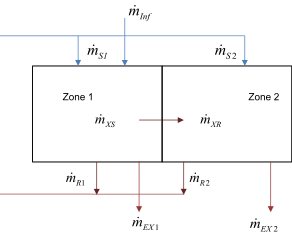
\includegraphics[width=0.9\textwidth, height=0.9\textheight, keepaspectratio=true]{media/image134.svg.png}
\caption{Illustration of zone air mass flow balance components \protect \label{fig:illustration-of-zone-air-mass-flow-balance}}
\end{figure}

An individual zone may be a source zone for multiple receiving zones, and the same source zone may receive mixing flows from multiple adjacent zones in an air loop. The source and receiving mass flow rates of ZoneMixing objects are calculated from user defined mixing flow rates at the first HVAC iteration for each time step and adjusted in subsequent iterations to balance the zone air mass flow. The source zone mixing mass flow rate is calculated by tracking the mass flow rates of ZoneMixing objects connected to a zone and is given by:

\begin{equation}
{\dot m_{XS}} = \sum\nolimits_j {{{\dot m}_{XS,j}}}
\end{equation}

Similarly, the receiving zone mixing mass flow rate is calculated by tracking the mass flow rates of ZoneMixing objects connected to a receiving zone and is given by:

\begin{equation}
{\dot m_{XR}} = \sum\nolimits_j {{{\dot m}_{XR,j}}}
\end{equation}

Zone air mass flow balance can be enforced using four options: \textit{AdjustMixingOnly}, \textit{AdjustReturnOnly}, \textit{AdjustMixingThenReturn}, or \textit{AdjustReturnThenMixing}.  These options involve either adjusting zone mixing objects flows, adjusting the zone total return air flows, or a 
combination of both. The zone air mass flow balance equation formulation for each of the four options is described next.

\textbf{AdjustMixingOnly:} adjusts the zone mixing object flows only to enforce zone air mass flow balance and the adjusted zone mixing mass flow rates are used to determine the zone total return air mass flow rate. Infiltration air flow can also adjusted if required depending on user preference as specified in Section \textit{Infiltration Flow rates Adjustments}.

Determine the zone total return air mass flow rate as shown above, then adjust the zone mixing mass flow rates based on the zone total return air mass flow rate:

\begin{equation}
{\dot m_{XR,\,new}} = {\dot m_R} + {\dot m_{EX}} + {\dot m_{XS}} - {\dot m_S}
\end{equation}

This updated receiving zone mixing air mass flow rate is distributed to the mixing objects connected to the current zone proportional to user specified design flow rate. A single zone may be connected to more than one adjacent zone using multiple ZoneMixing objects. Thus, the mixing flow rate of each contributing mixing objects defined in the current zone is updated as follows:

\begin{equation}
{\dot m_{XR,\,new,j}} = \left( {{{\dot m}_{XR,jDesign}}/{{\dot m}_{XR,Design}}} \right) \cdot {\dot m_{XR,\,new}}
\end{equation}

\textbf{AdjustReturnOnly:} adjusts the zone total return air mass flow rate only to enforce zone air mass flow balance while the zone mixing object mass flow rate are kept at user specified values. Infiltration air flow can also adjusted if required depending on user preference as specified in Section \textit{Infiltration Flow rates Adjustments}.

First, determine the user specified mixing object received and source air flow rates of the current zone, then determine the zone total return air flow rate as follows:

\begin{equation}
{\dot m_{XS}} = \sum\nolimits_j {{{\dot m}_{XS,j}}}
\end{equation}

\begin{equation}
{\dot m_{XR}} = \sum\nolimits_j {{{\dot m}_{XR,j}}}
\end{equation}

If ZoneAirMassFlowConservation is active, then determine the zone total return air flow rate:
\begin{equation}
{\dot m_{R}} = MAX\left( {0.0,\,{{\dot m}_S} - {{\dot m}_{EX,tot}} + [{{\dot m}_{XR}} - {{\dot m}_{XS}}]} \right)
\end{equation}

Also checks that the zone total return air mass flow rate does not exceed the airloop design supply flow rate as follows:
\begin{equation}
{\dot m_{R}} = MIN\left( {{\dot m_{R}},\,{{\dot m}_{DesSupply,i}}} \right) 
\end{equation}

\textbf{AdjustMixingThenReturn:} first adjusts the zone mixing air mass flow rates, then adjusts the zone total return air mass flow rate to enforce zone air mass flow balance. Infiltration air flow can also adjusted if required depending on user preference as specified in section \textit{Infiltration Flow rates Adjustments}. For adjusting the mixing mass flow rates the set of equations for \textit{AdjustMixingOnly} method described above are used and for adjusting the zone total return air mass flow rate the equation for \textit{AdjustReturnOnly} method is used. 

\textbf{AdjustReturnThenMixing:} first adjusts the zone total return air mass flow rate, then adjusts the zone mixing mass flow rates to enforce zone air mass flow balance. Infiltration air flow can also adjusted if required depending on user preference as specified in section \textit{Infiltration Flow rates Adjustments}. For adjusting the zone total return air mass flow rate the equation for \textit{AdjustReturnOnly} method described above is used and for adjusting the zone mixing mass flow rates the set of equations defined for \textit{AdjustMixingOnly} method are used.

\subsection{Infiltration Flow Rate Adjustments}\label{infiltration-flow-rate-adjustments}

There are three options for the treatement of infiltration in the zone air mass balance: None, AddInfiltrationFlow, and AdjustInfiltrationFlow. There are also two options to specify which zones are included in the infiltration adjustments: AllZones or MixingSourceZonesOnly.

If a zone is excluded from infiltration adjustments, then the base infiltration rate specified by the Infiltration:* object(s) in the zone is assumed to be self-balanced, and infiltration is not included in the mass flow calculations for that zone.

If a zone is included in the infiltration adjustment, the infiltration air mass flow rate required to balance the zone is determined as follows:

\begin{equation}
{\dot m_{Inf-required}} = MAX\left( {0.0,\,{{\dot m}_{XS}} + {{\dot m}_{EX}} + {{\dot m}_{R}} - {{\dot m}_S}  - {\dot m_{XR,\,new}}} \right)
\end{equation}

This infiltration air mass flow rate calculated is either added to the base infiltration air flow, which is calculated from user inputs, or overrides the base infiltration air flow depending on user choice. For AddInfiltrationFlow, the zoneinfiltration flow rate is:

\begin{equation}
{\dot m_{Inf}} = {\dot m_{Inf-base}} + {\dot m_{Inf-required}}
\end{equation}

For AdjustInfiltrationFlow, the zone infiltration flow rate is:

\begin{equation}
{\dot m_{Inf}} = {\dot m_{Inf-required}}
\end{equation}

where,

\({\dot m_{Inf}}\) = zone infiltration mass flow rate, (kg/s)

\({\dot m_{Inf-base}}\) = base zone infiltration mass flow rate calculated from Infiltration:* objects, (kg/s)

\({\dot m_{Inf-required}}\) = required zone infiltration mass flow rate to balance the zone, (kg/s)

There is an additional constraint to the return air mass flow rate calculation. The sum of the return air mass flow rates of zones in air loop must satisfy the air loop return air mass flow balance. The above four sets of equations are iterated for each zone in an air loop until the convergence criterion is satisfied or until the maximum iteration limit is exceeded.

The mass conservation calculations are performed in routine CalcZoneMassBalance in the ZoneEquipmentManager module. The latest ZoneMixing and Infiltration object flow rates are communicated back to the zone air heat balance terms. This is done by re-simulating the simple flow objects as zone equipment during each HVAC iteration. This requires calling the routine CalcAirFlowSimple in SimZoneEquipment routine as zone equipment. Both of these routines are also in the ZoneEquipmentManager module.

The zone mass conservation calculation convergence criterion is based on the absolute difference of the zone mixing objects mass flow rates between successive iteration. If the difference is above tolerance limits of 0.00001 then the HVAC Air loop is simulated again.
